
\documentclass[11pt,a4paper]{article}

% =====================================================
% PACOTES
% =====================================================
\usepackage[brazil]{babel}
\usepackage[utf8]{inputenc}
\usepackage[T1]{fontenc}
\usepackage[hmargin=21mm,vmargin=20mm]{geometry}

\usepackage{graphicx}
\usepackage{booktabs}
\usepackage{tabularx}
\usepackage{xcolor}
\usepackage{float}
\usepackage{placeins}
\usepackage{listings}

% =====================================================
% CONFIGURAÇÃO DE CÓDIGO
% =====================================================
\lstset{
    basicstyle=\ttfamily\footnotesize,
    breaklines=true,
    columns=fullflexible,
    keepspaces=true,
    inputencoding=utf8,
    extendedchars=true,
    literate={á}{{\'a}}1 {à}{{\`a}}1 {â}{{\^a}}1 {ã}{{\~a}}1
             {é}{{\'e}}1 {ê}{{\^e}}1 {í}{{\'i}}1 {ó}{{\'o}}1
             {ô}{{\^o}}1 {õ}{{\~o}}1 {ú}{{\'u}}1 {ç}{{\c{c}}}1
             {Á}{{\'A}}1 {À}{{\`A}}1 {Â}{{\^A}}1 {Ã}{{\~A}}1
             {É}{{\'E}}1 {Ê}{{\^E}}1 {Í}{{\'I}}1 {Ó}{{\'O}}1
             {Ô}{{\^O}}1 {Õ}{{\~O}}1 {Ú}{{\'U}}1 {Ç}{{\c{C}}}1
}

% =====================================================
% CORES
% =====================================================
\definecolor{cefetazul}{HTML}{173B5E}
\definecolor{cinzaescuro}{HTML}{444444}

% =====================================================
% LINKS E METADADOS
% =====================================================
\usepackage[
    colorlinks=true,
    linkcolor=teal!60!black,
    urlcolor=teal!60!black
]{hyperref}

\hypersetup{
    pdftitle={Disponibilidade de uma aplicação distribuída em Kubernetes},
    pdfauthor={Grupo G3 - CEFET-MG}
}

% =====================================================
% FORMATAÇÃO GERAL DO RELATÓRIO
% =====================================================
\setlength{\emergencystretch}{2em}
\setlength{\parskip}{2pt}
\setlength{\intextsep}{7pt}
\setlength{\abovecaptionskip}{6pt}
\setlength{\floatsep}{9pt}
\setlength{\textfloatsep}{10pt}

\widowpenalty=10000
\clubpenalty=10000

\renewcommand{\topfraction}{.94}
\renewcommand{\bottomfraction}{.85}
\renewcommand{\textfraction}{.06}
\renewcommand{\floatpagefraction}{.66}

\raggedbottom

% =====================================================
% INÍCIO DO DOCUMENTO
% =====================================================
\begin{document}

\hypersetup{pageanchor=false}

% =====================================================
% CAPA INSTITUCIONAL
% =====================================================
\begin{titlepage}
\thispagestyle{empty}
\centering

\vspace*{0.4cm}

% INSTITUIÇÃO
{\fontsize{15}{19}\selectfont\bfseries
UNIVERSIDADE FEDERAL DE CIÊNCIA\\
E INOVAÇÃO DE MINAS GERAIS\par}

\vspace{0.3cm}

{\normalsize
}

\vspace{1.1cm}

% LOGOTIPO
\IfFileExists{figuras/logo_ufci.jpeg}{
    
\includegraphics[
        width=0.32\textwidth,
        height=3.0cm,
        keepaspectratio
    ]{figuras/logo_ufci.jpeg}
}{
    \vspace{1.0cm}
}

\vspace{1.1cm}

% IDENTIFICAÇÃO DO TRABALHO
{\normalsize\bfseries
SISTEMAS OPERACIONAIS MODERNOS\par}

\vspace{0.5cm}

{\color{cefetazul}
\rule{\textwidth}{0.6pt}\par}

\vspace{0.5cm}

% TÍTULO
{\fontsize{23}{29}\selectfont\bfseries
Disponibilidade de uma\\
Aplicação Distribuída\\
em Kubernetes\par}

\vspace{0.45cm}

% SUBTÍTULO
{\fontsize{11.5}{16}\selectfont
Recuperação de Réplicas, Persistência de Dados\\
e Isolamento de Rede em um Cluster Local\par}

\vspace{0.5cm}

{\color{cefetazul}
\rule{\textwidth}{0.6pt}\par}

\vspace{0.7cm}

% INFORMAÇÕES DO PROJETO
{\normalsize
\textbf{Trabalho Prático de Orquestração}\\[0.2cm]
\textbf{Grupo G3 --- Tema 5}\\[0.3cm]
\textbf{Professor:} Michel Pires da Silva\par}

\vfill

% INTEGRANTES
{\normalsize\bfseries
DISCENTES\par}

\vspace{0.3cm}

{\fontsize{10.5}{15}\selectfont
Ahmed Amer Hachem\\
Bernardo Silva Andrade\\
Hugo Henrique Marques\\
João Pedro S. Siqueira\\
João Vitor Lobato Romualdo\\
Lucas Roseno Medeiros Araújo\\
Luiz Fernando Queiroz\\
Thallys Lamounier\par}

\vfill

% LOCAL E ANO
{\normalsize
\textbf{Divinópolis --- MG}\\
2026\par}

\vspace{0.3cm}

\end{titlepage}

% Reativar os links internos após a capa
\hypersetup{pageanchor=true}

% =====================================================
% MANTER A PARTIR DAQUI O SUMÁRIO E O RELATÓRIO
% =====================================================

\hypersetup{pageanchor=true}
\tableofcontents\clearpage
\FloatBarrier\section{Introdução}
Para quem utiliza um serviço que registra operações, receber uma página e conseguir concluir uma operação são experiências distintas. Uma interface pode permanecer acessível enquanto a aplicação perdeu a capacidade de gravar. Essa distinção orientou a análise de uma aplicação web de contagem de visitas: a cada consulta, o cliente consegue observar qual instância respondeu e se a visita foi registrada. O serviço expõe, assim, dois efeitos de uma falha que um teste restrito ao código HTTP poderia confundir.

A conteinerização permite iniciar outra instância do programa a partir da mesma imagem. Para recuperar o serviço, porém, também é preciso detectar a ausência da instância, iniciar sua substituta e decidir quando encaminhar tráfego a ela. Há ainda um problema de estado: se cada cópia mantivesse a contagem apenas em sua memória, remover uma réplica eliminaria parte do histórico e consultar outra produziria um total diferente. No projeto, o Kubernetes gerencia a quantidade de instâncias da aplicação, e o PostgreSQL mantém o registro comum às réplicas em um volume que pode ser remontado após a substituição do pod.

O objetivo geral foi avaliar até onde essa divisão de responsabilidades preserva o atendimento diante de mudanças no cluster. Os objetivos específicos foram verificar a distribuição das chamadas entre réplicas, medir a reposição após uma remoção, observar a expansão manual e automática, acompanhar o contador durante a recriação do banco e testar quais clientes conseguem alcançar sua porta. Os ensaios complementares verificaram o efeito de uma imagem indisponível e a possibilidade de iniciar componentes com imagens já presentes no nó.

A arquitetura é examinada a seguir pelo percurso de uma visita. A análise experimental separa a observação feita pelo cliente da observação dos controladores. O escopo é um laboratório Minikube de nó único: ele permite provocar a perda de um pod conservando o restante do ambiente. Esse desenho define tanto as conclusões possíveis quanto os limites de sua transferência a um serviço distribuído entre máquinas.

\FloatBarrier\section{Mapeamento da Solução e Arquitetura}
O navegador carrega um painel que consulta periodicamente a rota de identificação da API. O endereço usado pelo cliente permanece estável quando um pod é substituído. Isso é possível porque o Service da aplicação recebe conexões pela porta publicada no nó e encaminha o tráfego para pods selecionados por rótulo. O processo HTTP recebe a conexão na porta interna do contêiner. A Figura~\ref{fig:arquitetura} acompanha a consulta que resulta em escrita.
\begin{figure}[!ht]\centering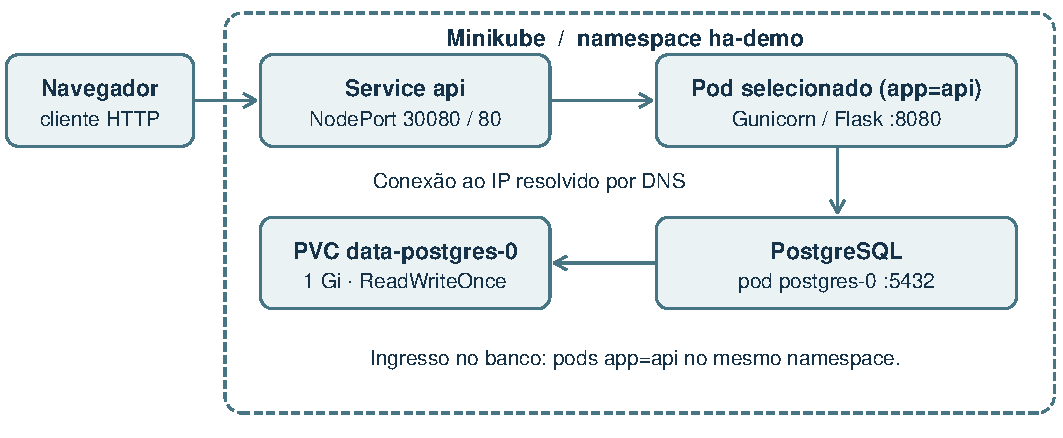
\includegraphics[width=\linewidth]{figuras/arquitetura-final.pdf}
\caption{Percurso de uma visita a partir dos objetos declarados no projeto. A seta entre API e banco representa a conexão aberta após a descoberta do endereço pelo Service interno. A seta para o PVC representa a montagem do armazenamento.}\label{fig:arquitetura}\end{figure}

Cada réplica obtém do Kubernetes sua identidade, seu IP e o nome do nó. Ao receber a consulta, a aplicação abre uma conexão ao PostgreSQL por nome de serviço, insere uma linha com a identificação do pod e lê a quantidade de linhas. A resposta combina dados locais, como a identidade de quem atendeu, com um dado compartilhado, a contagem. Fechar a conexão HTTP após a resposta dá à próxima conexão outra oportunidade de seleção de destino. A escolha pode voltar ao mesmo pod. Por isso, a alternância de identidades é uma observação mais informativa que a expectativa de uma ordem circular fixa.

O Service do banco é interno e do tipo \textit{headless}: oferece descoberta por DNS para alcançar o pod do PostgreSQL. A política de ingresso permite a porta do banco aos pods com o rótulo da aplicação no mesmo namespace. Há duas verificações em camadas diferentes: alcançar a porta permite iniciar a comunicação, enquanto executar a escrita exige uma sessão válida no banco. O PostgreSQL mantém seus arquivos num volume reservado ao primeiro membro do StatefulSet. Um pod recriado com a mesma identidade ordinal pode remontar esse volume e abrir o conjunto de dados existente.

A Figura~\ref{fig:objetos} detalha a distribuição das responsabilidades. Cada pod da API contém o processo de atendimento e um contêiner de inicialização que termina antes dele. Os parâmetros comuns chegam pelo ConfigMap e pelo Secret. O Service seleciona as réplicas disponíveis; o Deployment governa sua quantidade. Na camada persistente, o StatefulSet postgres gerencia o pod postgres-0 e associa sua identidade ordinal ao claim data-postgres-0 (ambos representados na faixa inferior do diagrama). As setas de configuração e controle não representam tráfego de visitas.

\begin{figure}[!ht]\centering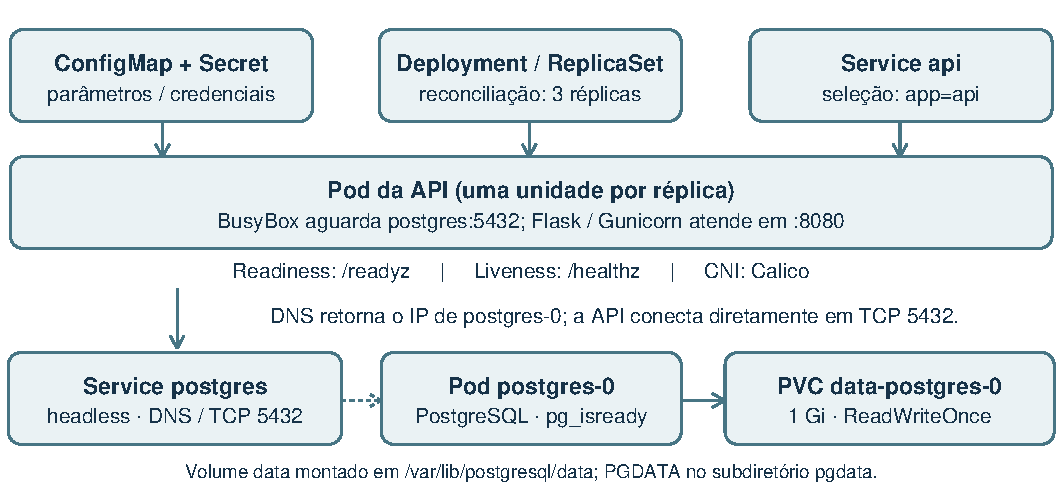
\includegraphics[width=\linewidth]{figuras/objetos-final.pdf}\caption{Arquitetura dos componentes Kubernetes utilizados no projeto. As setas superiores indicam, respectivamente, injeção de configuração, controle de réplicas e encaminhamento HTTP. O trecho pontilhado inferior identifica o pod postgres-0 (gerenciado pelo StatefulSet postgres e vinculado ao PVC data-postgres-0) descoberto pelo Service headless. A API verifica prontidão em /readyz e vivacidade em /healthz.}\label{fig:objetos}\end{figure}

O momento da falha também importa. Antes de iniciar a API, um contêiner de inicialização espera que a porta do banco aceite conexão. Após a inicialização, a sonda de prontidão da API verifica o servidor web independentemente do banco. Se uma gravação falhar, a aplicação ainda consegue devolver a identidade do pod e indicar que a contagem está indisponível. Portanto, uma queda do banco pode permitir atendimento parcial pelas réplicas existentes e simultaneamente retardar a entrada de novas réplicas. A segunda consequência decorre da configuração de inicialização; o comportamento registrado durante a queda é discutido na Seção~\ref{sec:dados}.

A arquitetura dispõe de várias réplicas HTTP, mas concentra as escritas em uma instância do PostgreSQL. Recriar essa instância sobre o volume existente exige um intervalo de inicialização. Também há dependência do nó que executa o laboratório. São duas fronteiras de falha diferentes daquela exercitada ao remover apenas uma réplica HTTP.

\FloatBarrier\section{Tecnologias Utilizadas}
\paragraph{Empacotamento e execução:} A imagem da aplicação reúne Python, Flask, Gunicorn e o cliente PostgreSQL. Flask implementa as rotas e constrói a resposta. Gunicorn recebe conexões e distribui o trabalho entre processos e threads dentro de cada réplica. Essa concorrência local é distinta da escala do Kubernetes, que acrescenta pods completos ao conjunto atendido pelo Service. O cliente psycopg abre a conexão usada para a operação SQL. Na implementação atual, a conexão é obtida por requisição, o que permite uma nova tentativa em consulta posterior à recuperação do banco.

\paragraph{Orquestração e configuração:} Minikube fornece o ambiente local em que é possível observar o ciclo de vida dos pods. O Deployment declara a quantidade desejada de réplicas da API e usa um ReplicaSet para mantê-la. O StatefulSet atende a outra necessidade: associar a instância do PostgreSQL a uma identidade e a uma solicitação de volume estáveis. O ConfigMap distribui parâmetros compartilhados, enquanto o Secret fornece os valores de autenticação aos consumidores. A Downward API entrega os dados individuais de cada pod. Essa combinação permite que instâncias originadas da mesma imagem se identifiquem de forma distinta ao cliente.

\paragraph{Saúde, isolamento e elasticidade:} BusyBox executa a espera inicial por TCP e também fornece ferramentas leves aos pods de teste. O kubelet consulta sondas distintas para decidir se o processo deve receber tráfego ou ser reiniciado. No PostgreSQL, as sondas usam a ferramenta de prontidão do próprio banco. O Calico aplica as regras de rede entre pods. Para a escala automática, o metrics-server fornece medidas de recursos e o controlador HPA ajusta o tamanho do Deployment de acordo com a utilização média de CPU. O HPA é opcional: mantê-lo separado da implantação base permite atribuir a expansão manual à ação do operador e a expansão sob carga à decisão do controlador.
\paragraph{Unidades de execução:} Dentro de cada pod da API, o contêiner BusyBox termina sua verificação antes que o contêiner da aplicação inicie. Só este último atende ao navegador. Já o pod temporário de carga permanece ativo durante o ensaio do HPA e gera as requisições que provocam consumo de CPU. A separação permite encerrar a carga sem reiniciar os servidores. Os clientes de teste da política de rede têm outra finalidade: variar o rótulo de origem enquanto se mantém o destino PostgreSQL.

\paragraph{Coordenação entre controladores:} O Deployment ajusta o número de réplicas por meio do ReplicaSet, enquanto o Service encaminha conexões aos pods aptos. O StatefulSet preserva a associação entre a identidade do banco e o PVC durante a recriação.

\section{Execução e Validação Experimental}
\label{sec:validacao}

Os experimentos foram conduzidos em uma estação host Linux Ubuntu 24.04.4 LTS (kernel \texttt{6.14.0-33-generic}, \texttt{x86\_64}) executando o cluster Minikube \texttt{v1.39.0} (Kubernetes \texttt{v1.37.0}, runtime \texttt{containerd 2.3.4} e plugin CNI Calico). Os ensaios de autorrecuperação, escala e persistência foram repetidos em $n = 5$ rodadas. Os resultados estão na Tabela~\ref{tab:resultados-experimentais}.

\begin{table*}[t]
\centering
\caption{Resultados Quantitativos dos Ensaios de Autorrecuperação, Escalabilidade Horizontal e Persistência Transacional ($n = 5$)}
\label{tab:resultados-experimentais}
\scriptsize
\setlength{\tabcolsep}{1.8pt}
\begin{tabular*}{\textwidth}{@{\extracolsep{\fill}}c cccc c cccc@{}}
\toprule
 & \multicolumn{4}{c}{\textbf{1. Autorrecuperação de Pod (\texttt{selfheal.csv})}} & \multicolumn{1}{c}{\textbf{2. Escala (\texttt{scale.csv})}} & \multicolumn{4}{c}{\textbf{3. Persistência no PostgreSQL (\texttt{persistencia.csv})}} \\
\cmidrule(lr){2-5} \cmidrule(lr){6-6} \cmidrule(l){7-10}
\textbf{Rodada} & \textbf{\texttt{3/3 Ready} (s)} & \textbf{Erros} & \textbf{Reqs.} & \textbf{Sucesso (\%)} & \textbf{\texttt{3$\rightarrow$10 Ready} (s)} & \textbf{Antes} & \textbf{Depois} & \textbf{$\Delta$} & \textbf{Retenção} \\
\midrule
1 & 5,96 & 0 & 34 & 100,00\% & 7,16 & 314 & 315 & $+1$ & 100\% (0 perda) \\
2 & 5,84 & 1 & 34 & 97,06\%  & 6,58 & 260 & 261 & $+1$ & 100\% (0 perda) \\
3 & 8,84 & 0 & 40 & 100,00\% & 6,82 & 282 & 283 & $+1$ & 100\% (0 perda) \\
4 & 8,83 & 0 & 37 & 100,00\% & 6,80 & 502 & 503 & $+1$ & 100\% (0 perda) \\
5 & 8,38 & 0 & 37 & 100,00\% & 6,75 & 524 & 525 & $+1$ & 100\% (0 perda) \\
\midrule
\textbf{Média $\pm$ DP} & $\mathbf{7{,}57 \pm 1{,}54\,\textbf{s}}$ & $\mathbf{0{,}20 \pm 0{,}45}$ & $\mathbf{36{,}40 \pm 2{,}51}$ & $\mathbf{99{,}45\%\ (181/182)}$ & $\mathbf{6{,}82 \pm 0{,}21\,\textbf{s}}$ & --- & --- & $\mathbf{+1{,}00 \pm 0{,}00}$ & $\mathbf{100\%\ (5/5)}$ \\
\bottomrule
\end{tabular*}
\end{table*}

\subsection{Balanceamento de Carga e Exposição via NodePort}
A validação do plano de dados em regime nominal iniciou-se com a inspeção das 3 réplicas do \texttt{Deployment api} (\texttt{api-58cf7fff8c-8kbgh}, \texttt{b5mqd} e \texttt{qtbx5}), alocadas na sub-rede \texttt{10.244.120.70}--\texttt{72} e vinculadas ao objeto \texttt{Endpoints} do serviço \texttt{api} (\texttt{NodePort 10.99.68.112}, mapeamento \texttt{80:30080/TCP}). Em razão do encerramento explícito de conexões TCP a cada resposta (\texttt{Connection: close} e \texttt{keepalive = 0}), uma sequência de 20 requisições consecutivas a \texttt{/api/whoami} (\texttt{relatorio/logs/17-r4.txt}) demonstrou alternância efetiva entre os três backends pelas regras \texttt{iptables} do \texttt{kube-proxy}, enquanto o contador transacional \texttt{visits} progrediu monotonamente de \texttt{21} a \texttt{40}:

\begin{lstlisting}
NAME  TYPE      CLUSTER-IP    PORT(S)       AGE
api   NodePort  10.99.68.112  80:30080/TCP  85s
NAME  ENDPOINTS
api   10.244.120.70:8080,10.244.120.71:8080,
      10.244.120.72:8080
# Sequencia de respostas (pod / db / visits):
api-58cf7fff8c-b5mqd   ok   23
api-58cf7fff8c-8kbgh   ok   24
api-58cf7fff8c-b5mqd   ok   25
api-58cf7fff8c-8kbgh   ok   28
api-58cf7fff8c-qtbx5   ok   31
api-58cf7fff8c-qtbx5   ok   39
\end{lstlisting}

A Figura~\ref{fig:r4-pagina} apresenta a interface web de monitoramento servida pela aplicação durante o teste, evidenciando a detecção simultânea das três réplicas (\texttt{8kbgh}, \texttt{b5mqd} e \texttt{qtbx5}), latência média de $16\,\text{ms}$, ausência de falhas HTTP e distribuição equilibrada na barra histórica das últimas 40 respostas.

\begin{figure}[t]
\centering
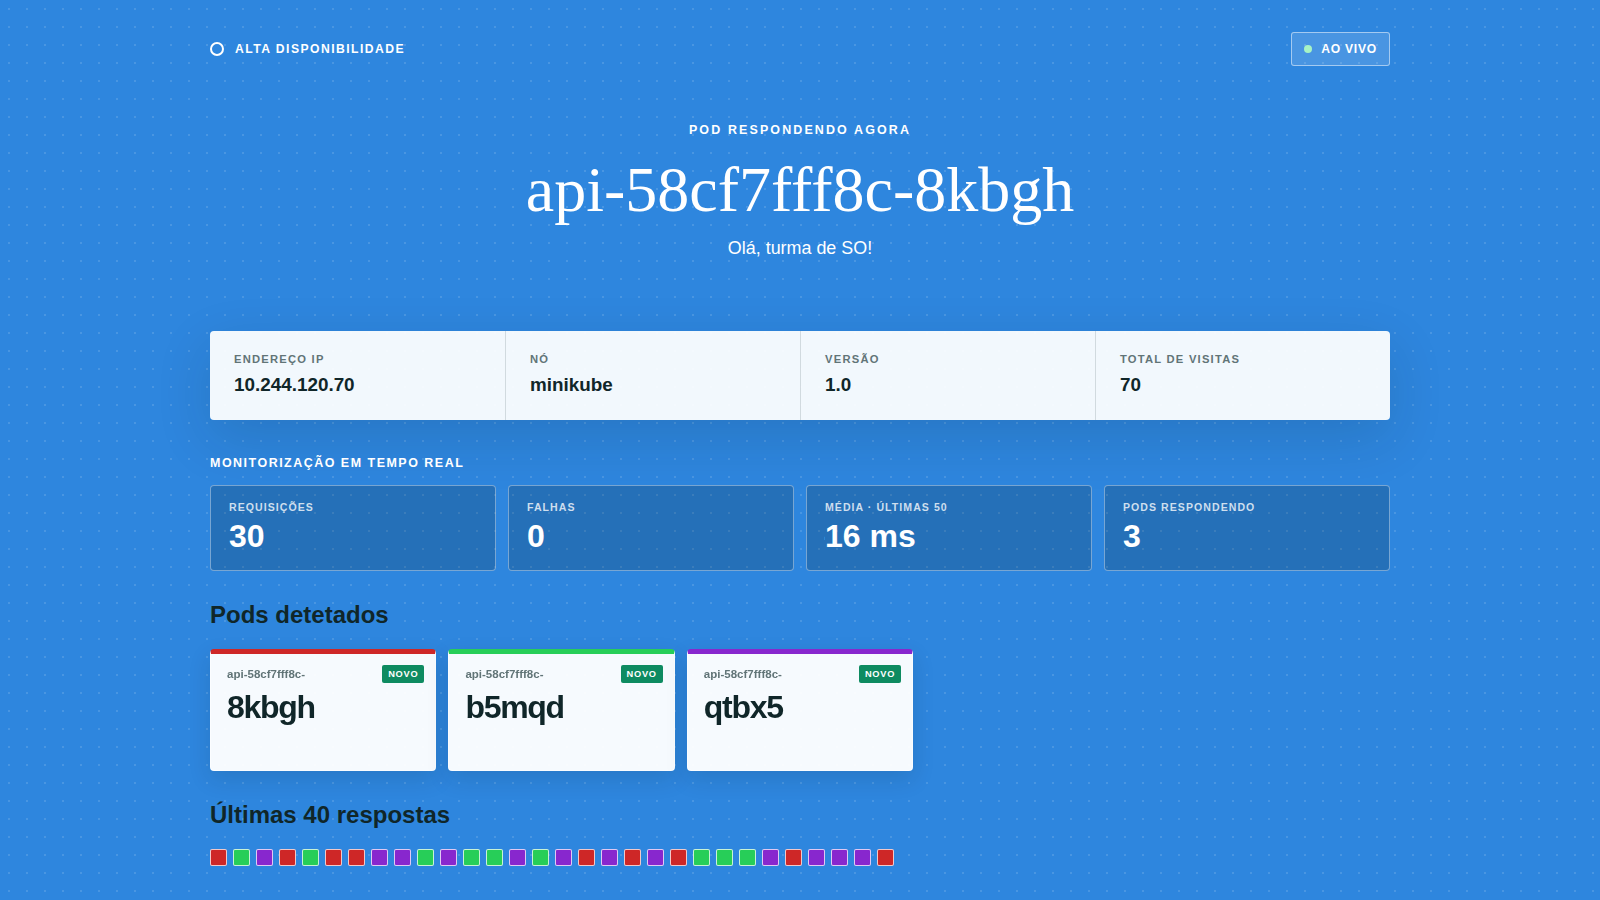
\includegraphics[width=0.84\columnwidth]{figuras/17-r4-pagina.png}
\caption{Painel de telemetria em operação nominal com 3 réplicas ativas (\texttt{8kbgh}, \texttt{b5mqd} e \texttt{qtbx5}), latência média de $16\,\text{ms}$ e balanceamento de carga L4 entre os pods.}
\label{fig:r4-pagina}
\end{figure}

\subsection{Autorrecuperação (\textit{Self-Healing}) de Pods e de Processo}
A resiliência da camada de aplicação foi avaliada sob duas modalidades de injeção de falhas:
\begin{enumerate}
    \item \textbf{Remoção abrupta de pod (\texttt{kubectl delete pod}):} A exclusão da réplica \texttt{api-58cf7fff8c-8kbgh} (\texttt{UID 3464f481-...}) sensibilizou imediatamente o laço de reconciliação do controlador \texttt{ReplicaSet} no \texttt{kube-controller-manager}. Ao detectar a divergência entre \texttt{spec.replicas: 3} e apenas 2 réplicas ativas, o controlador emitiu o evento \texttt{SuccessfulCreate} para o pod substituto \texttt{api-58cf7fff8c-wbgrv} (\texttt{IP 10.244.120.77}) no mesmo segundo em que o pod original entrou em estado \texttt{Killing}/\texttt{Terminating}, restabelecendo a condição \texttt{3/3 Ready} em $5897\,\text{ms}$. A Figura~\ref{fig:r5-transicao} ilustra, via \texttt{kubectl get pods -n ha-demo -w}, a transição completa de estados no kernel e no runtime (\texttt{Terminating} $\rightarrow$ \texttt{Pending} $\rightarrow$ \texttt{Init:0/1} $\rightarrow$ \texttt{PodInitializing} $\rightarrow$ \texttt{Running 1/1} em $5\,\text{s}$ na réplica substituta \texttt{9xwwk}). Nas $n = 5$ execuções automatizadas com sondagem HTTP a cada $100\,\text{ms}$ (Tabela~\ref{tab:resultados-experimentais}), o tempo médio de convergência até \texttt{3/3 Ready} foi de $7{,}57 \pm 1{,}54\,\text{s}$, com taxa global de disponibilidade HTTP de $99{,}45\%$ ($181/182$ requisições bem-sucedidas, registrando-se um único erro transitório na Rodada 2 durante a janela sub-segundo de atualização das regras \texttt{iptables}).
    \item \textbf{Travamento lógico de processo (\texttt{POST /api/crash}):} A criação do arquivo sentinela \texttt{/tmp/unhealthy} faz com que a rota \texttt{GET /healthz} passe a retornar HTTP \texttt{500}. Após \texttt{failureThreshold: 3} verificações consecutivas da \texttt{livenessProbe} (\texttt{periodSeconds: 5}, totalizando $\approx 15\,\text{s}$), o agente \texttt{kubelet} reinicia o container \texttt{api} in-loco, incrementando o contador \texttt{RESTARTS} sem alterar o \texttt{POD\_NAME} ou o \texttt{POD\_IP} e limpando o sistema de arquivos efêmero do container.
\end{enumerate}

\begin{figure}[t]
\centering
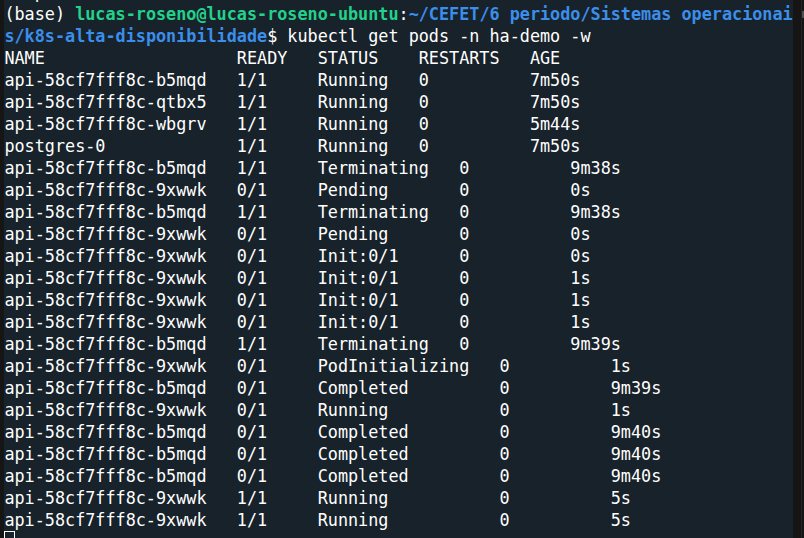
\includegraphics[width=0.84\columnwidth]{figuras/17-r5-transicao.png}
\caption{Captura em tempo real (\texttt{kubectl get pods -n ha-demo -w}) do ciclo de autorrecuperação: transição \texttt{Terminating} $\rightarrow$ \texttt{Pending} $\rightarrow$ \texttt{Init:0/1} $\rightarrow$ \texttt{PodInitializing} $\rightarrow$ \texttt{Running 1/1} em $5\,\text{s}$.}
\label{fig:r5-transicao}
\end{figure}

\subsection{Elasticidade Horizontal Imperativa ($3 \rightarrow 10$ Réplicas) e Reativa (\texttt{HPA})}
\begin{itemize}
    \item \textbf{Escalonamento Imperativo e Teste de Estresse Concorrente:} O disparo de \texttt{kubectl scale deployment api -n ha-demo -{}-replicas=10} instanciou 7 novas réplicas (\texttt{96rnn}, \texttt{9d74k}, \texttt{cggt4}, \texttt{j9hk2}, \texttt{k2fcw}, \texttt{kxzrl} e \texttt{qwrrm}, IPs \texttt{10.244.120.78}--\texttt{84}), atingindo \texttt{10/10 Ready} em $6{,}82 \pm 0{,}21\,\text{s}$ na média das 5 execuções (Tabela~\ref{tab:resultados-experimentais}). O baixo desvio-padrão decorre da retenção local das imagens OCI no \texttt{containerd} e da prontidão imediata do serviço \texttt{postgres} no \texttt{initContainer}. A Figura~\ref{fig:r6-dez-pods} exibe o painel web com os 10 pods respondendo simultaneamente e latência média reduzida para $13\,\text{ms}$. Submetido a uma bateria de estresse de $3000$ requisições concorrentes (20 clientes paralelos via \texttt{xargs -P 20}), o conjunto de 10 réplicas (40 \textit{threads} Gunicorn) processou $100\%$ das chamadas ($3000/3000$) com \texttt{\textquotedbl{}db\textquotedbl{}:\textquotedbl{}ok\textquotedbl{}}, enquanto o pod \texttt{postgres-0} operou em $172\,\text{mCPU}$ e $39\,\text{MiB}$ de RAM, abaixo dos seus limites de \texttt{cgroups} (\texttt{250m}/\texttt{512Mi}).
    \item \textbf{Autoescalonamento Reativo via \texttt{HPA}:} Em repouso, \texttt{kubectl top pods} indicou consumo de $2\,\text{mCPU}$ e $76\,\text{MiB}$ por réplica da API (\texttt{TARGETS: cpu: 2\%/50\%}). Com a ativação do gerador de carga \texttt{scripts/load-hpa.sh} (6 fluxos concorrentes em \texttt{/api/cpu?ms=200}), a utilização média subiu a $230\%$ do \texttt{request} ($113\text{--}143\,\text{mCPU}$ por pod), levando o \texttt{HPA} a expandir o \texttt{Deployment} progressivamente de $3 \rightarrow 6 \rightarrow 10$ réplicas em $30\,\text{s}$, diluindo a carga média para $133\%$ (\texttt{4m45s}):
\end{itemize}

\begin{lstlisting}
$ kubectl get hpa -n ha-demo -w
NAME REFERENCE      TARGETS       MIN MAX REPLICAS AGE
api  Deployment/api cpu: 2%/50%   3   10  3        80s
api  Deployment/api cpu: 230%/50% 3   10  3        2m45s
api  Deployment/api cpu: 230%/50% 3   10  6        3m
api  Deployment/api cpu: 230%/50% 3   10  10       3m15s
api  Deployment/api cpu: 133%/50% 3   10  10       4m45s
# Apos encerrar carga (estabilizacao de 300s):
api  Deployment/api cpu: 2%/50%   3   10  10       31m
api  Deployment/api cpu: 2%/50%   3   10  3        35m
\end{lstlisting}

\begin{figure}[t]
\centering
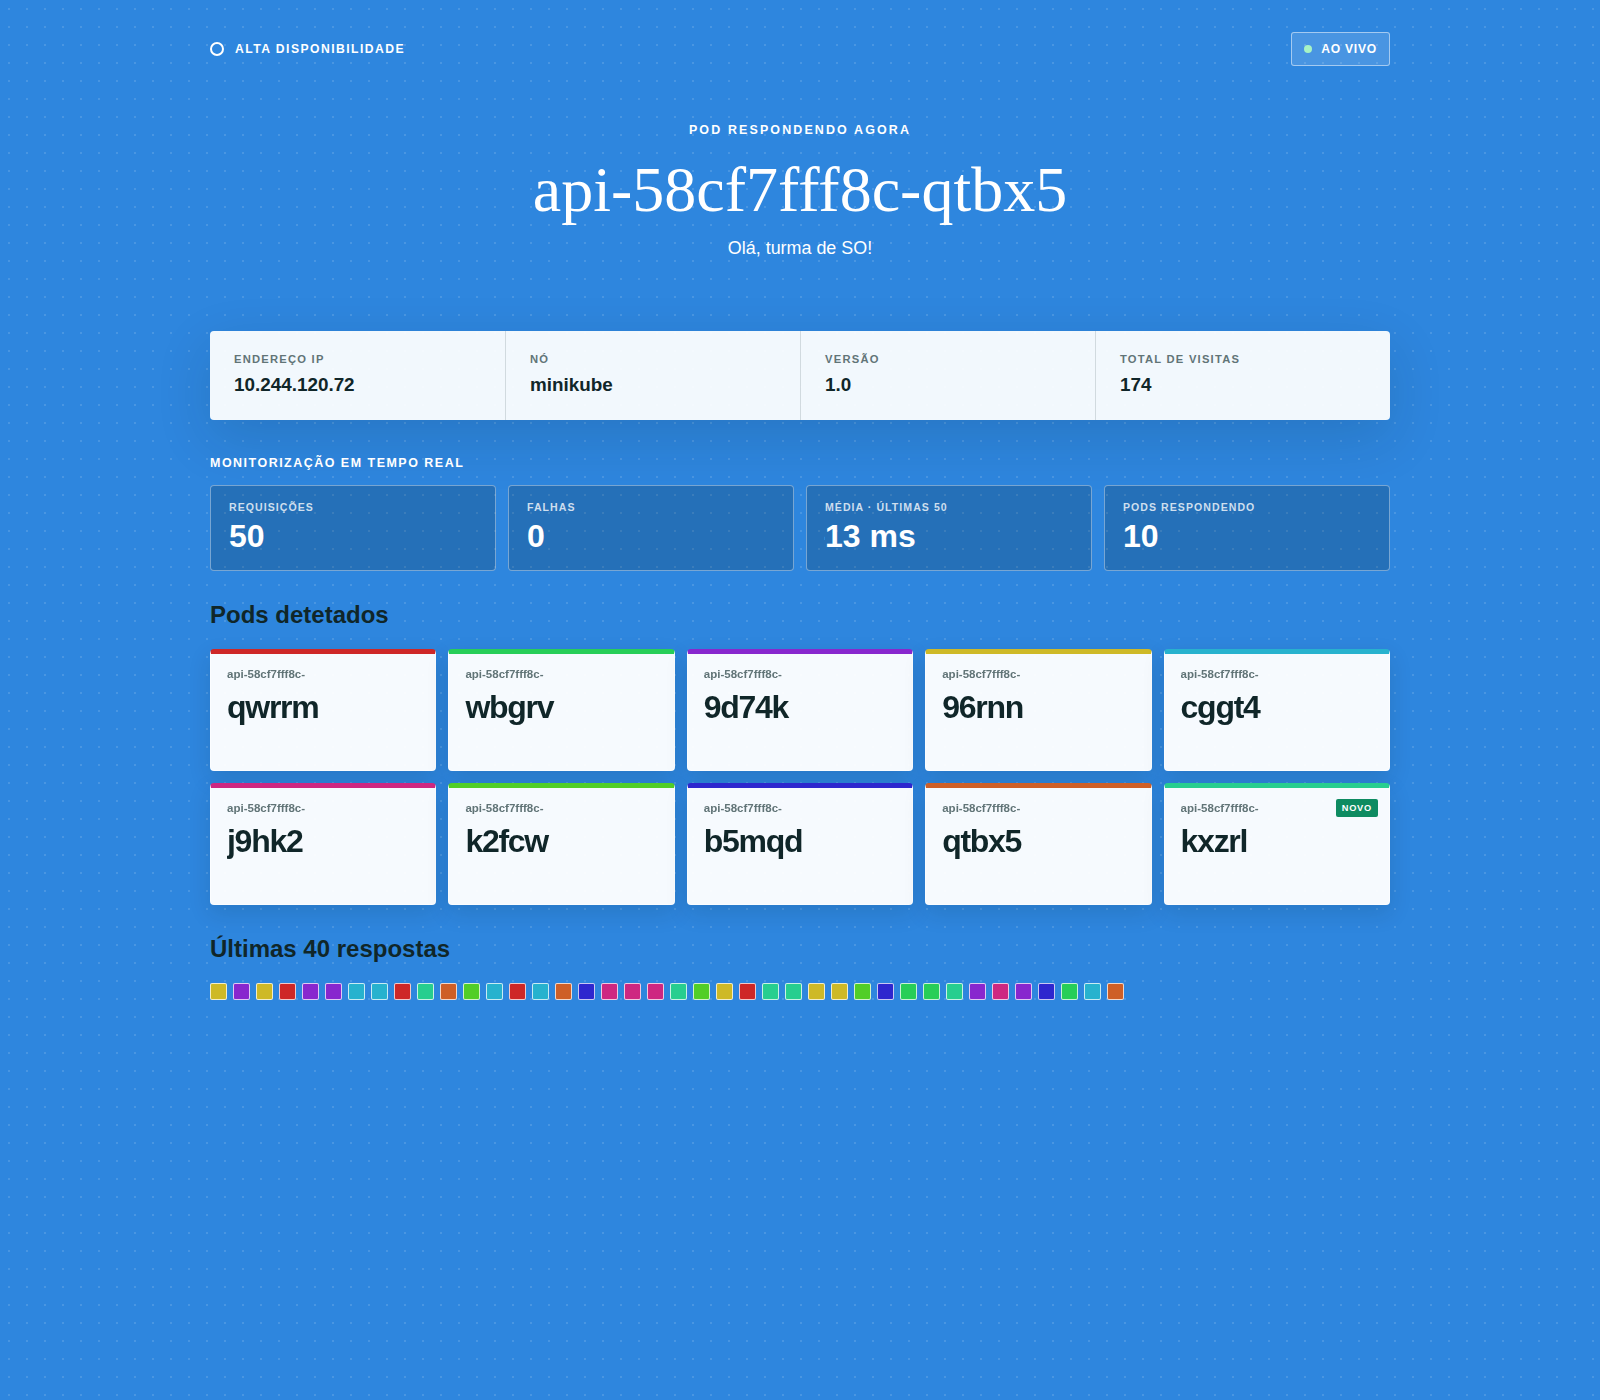
\includegraphics[width=0.84\columnwidth]{figuras/17-r6-dez-pods.png}
\caption{Painel web após escalonamento horizontal para 10 réplicas ativas no namespace \texttt{ha-demo}, operando com zero falhas e latência média de $13\,\text{ms}$.}
\label{fig:r6-dez-pods}
\end{figure}

\subsection{Persistência Transacional, Degradação Graciosa, Isolamento de Rede e Operação Offline}
\begin{itemize}
    \item \textbf{Persistência em \texttt{StatefulSet}/\texttt{PVC} e Degradação Graciosa:} Na Rodada 1 da Tabela~\ref{tab:resultados-experimentais}, após acumular \texttt{visits: 314}, o pod \texttt{postgres-0} foi removido (\texttt{kubectl delete pod postgres-0 -n ha-demo}). Durante os $7\,\text{s}$ de recriação do container pelo \texttt{StatefulSet}, chamadas a \texttt{/api/whoami} retornaram \texttt{HTTP/1.1 200 OK} com payload degradado (\texttt{\textquotedbl{}visits\textquotedbl{}:null, \textquotedbl{}db\textquotedbl{}:\textquotedbl{}indisponível\textquotedbl{}}). Graças ao desacoplamento da sonda \texttt{GET /readyz}, as 3 réplicas da API permaneceram ativas no \texttt{Service}, e o painel web (Figura~\ref{fig:painel-banco-fora}) exibiu o alerta \textquotedbl{}BANCO FORA DO AR\textquotedbl{} preservando em tela a última contagem válida sem erros HTTP. Concluída a prontidão do novo \texttt{postgres-0}, o volume \texttt{data-postgres-0} manteve exatamente o mesmo identificador (\texttt{UID 873f564d-32f8-4e88-8472-cb408247b7b9}) e a requisição seguinte registrou \texttt{visits: 315} (\texttt{\textquotedbl{}db\textquotedbl{}:\textquotedbl{}ok\textquotedbl{}}), comprovando retenção integral do estado em todas as 5 execuções ($\Delta = +1$).
    \item \textbf{Isolamento de Rede via Calico \texttt{NetworkPolicy}:} Com a política \texttt{postgres-allow-api} ativa, um pod efêmero sem o rótulo autorizado (\texttt{kubectl run intruso -{}-image=busybox:1.36}) teve pacotes SYN descartados pelo \textit{netfilter} ao testar a porta \texttt{5432} (\texttt{nc: postgres (10.244.54.229:5432): Connection timed out}, código de saída \texttt{1}), enquanto um pod rotulado com \texttt{app=api} (\texttt{amigo}) estabeleceu conexão TCP imediata (\texttt{postgres (10.244.54.229:5432) open}, saída \texttt{0}).
    \item \textbf{Atualização Contínua (\textit{Rolling Update}) e Operação 100\% Offline:} A substituição gradual de versão na API sob \texttt{maxSurge: 1} e \texttt{maxUnavailable: 0} manteve 100\% de disponibilidade durante a transição. Por fim, bloqueando-se todo o tráfego externo de internet no nó Minikube via regras \texttt{iptables REJECT} nas cadeias \texttt{OUTPUT} e \texttt{FORWARD} (confirmado pela falha de conexão a \texttt{https://registry-1.docker.io/v2/}), a recriação completa do ambiente (\texttt{reset.sh} + \texttt{deploy.sh}) e a exclusão forçada do \texttt{postgres-0} convergiram para \texttt{Running 1/1} em $6\text{--}12\,\text{s}$ com eventos \texttt{Pulled: Container image already present on machine}, validando a autonomia offline proporcionada por \texttt{imagePullPolicy: IfNotPresent}.
\end{itemize}

\begin{figure}[t]
\centering
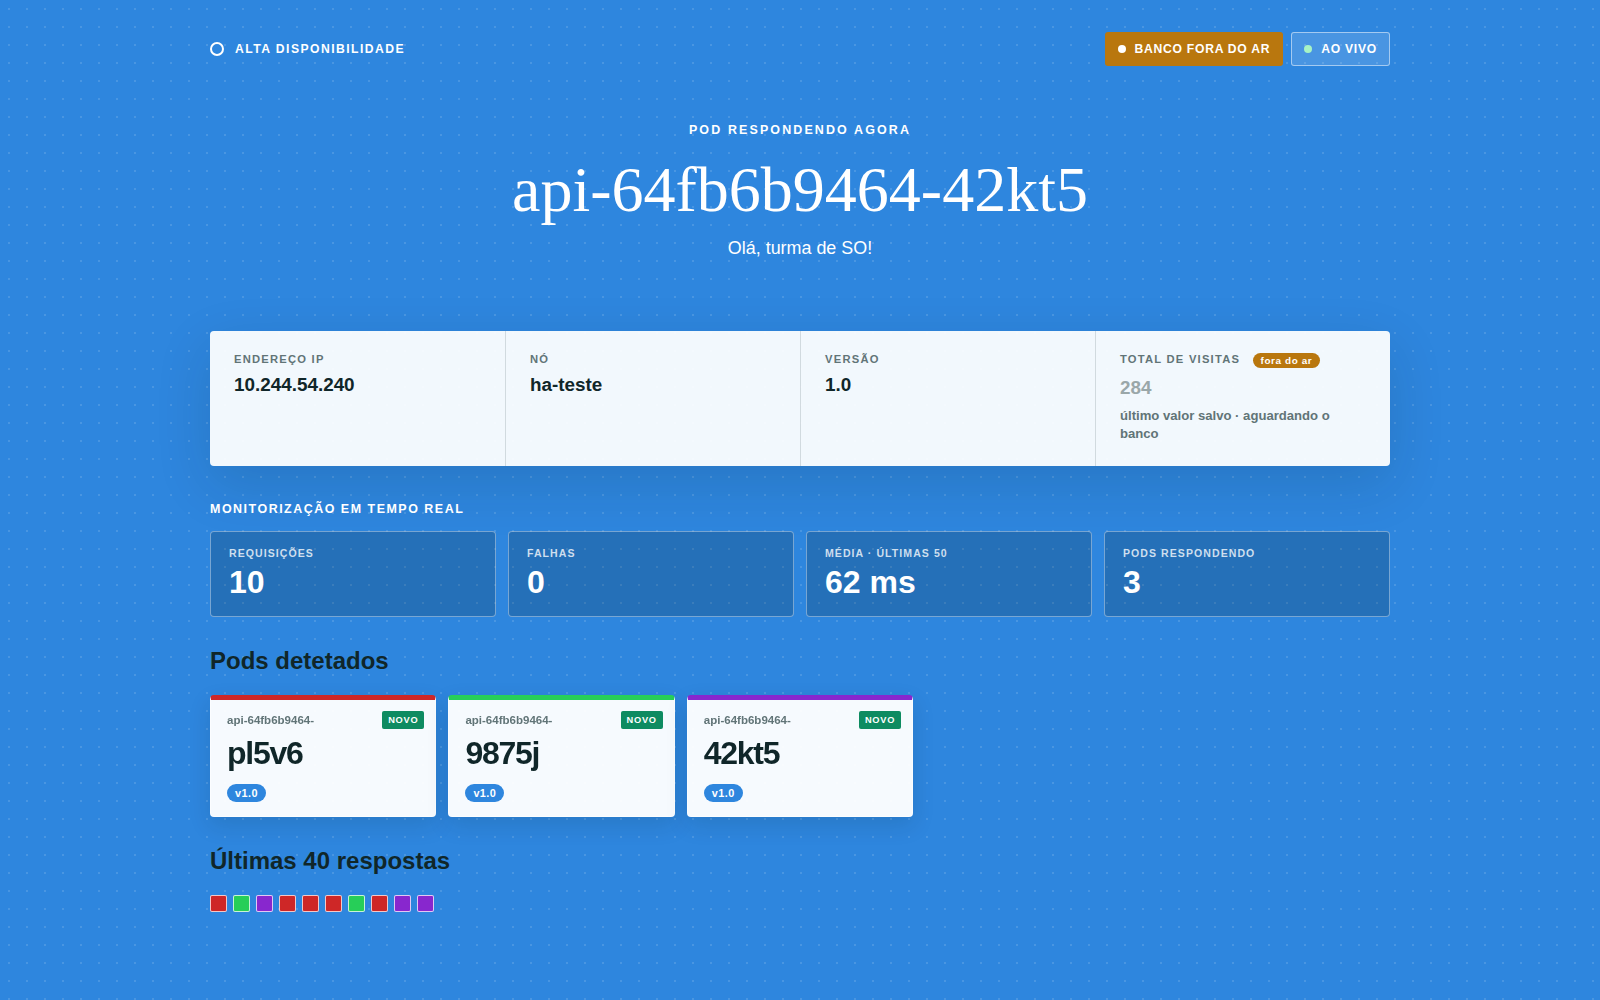
\includegraphics[width=0.84\columnwidth]{figuras/22-painel-banco-fora.png}
\caption{Degradação graciosa no painel de telemetria durante a recriação do pod \texttt{postgres-0}: sinalização \textquotedbl{}BANCO FORA DO AR\textquotedbl{}, preservação do último contador em cache (\texttt{284}) e zero falhas HTTP nas 3 réplicas da API.}
\label{fig:painel-banco-fora}
\end{figure}

\FloatBarrier\section{Conclusão}


O desenvolvimento deste trabalho permitiu analisar, na prática, o funcionamento de uma aplicação distribuída gerenciada pelo Kubernetes, com ênfase na disponibilidade dos serviços, na recuperação automática de falhas e na escalabilidade. Os experimentos demonstraram que, diante da remoção de uma réplica da aplicação, o orquestrador foi capaz de identificar a alteração e iniciar sua substituição, restabelecendo a quantidade de três instâncias configuradas. Esse comportamento evidenciou o mecanismo de autorrecuperação (\textit{self-healing}) e a importância da manutenção do estado desejado para a continuidade do atendimento.

Os testes de escalabilidade também demonstraram a flexibilidade proporcionada pela orquestração. A expansão manual de três para dez réplicas comprovou a possibilidade de aumentar a quantidade de instâncias da aplicação por meio de uma alteração na configuração desejada. Complementarmente, o escalonamento automático, realizado com o Horizontal Pod Autoscaler (HPA), evidenciou a capacidade do Kubernetes de ajustar a quantidade de réplicas em resposta à utilização de CPU. Esses resultados permitiram compreender a diferença entre o gerenciamento manual de recursos e a adaptação automática da infraestrutura às condições de carga observadas.

A integração com o PostgreSQL e os experimentos de persistência e isolamento de rede ampliaram a compreensão sobre as dependências existentes entre os componentes de um sistema distribuído. Durante a recriação do banco de dados, a aplicação continuou respondendo às requisições HTTP, embora as operações de gravação estivessem temporariamente indisponíveis. Após a recuperação, a contagem de visitas foi retomada a partir dos valores anteriormente registrados, demonstrando a importância do armazenamento persistente. Os testes de política de rede também evidenciaram como o controle da comunicação entre os serviços contribui para a organização e a segurança da infraestrutura.

Dessa forma, a realização dos experimentos proporcionou à equipe um aprendizado sobre a gestão de sistemas interconectados. Foi possível compreender que a disponibilidade de uma aplicação não depende apenas da existência de contêineres em execução, mas também da comunicação entre os serviços, do funcionamento das dependências e da configuração adequada dos mecanismos de recuperação. Além disso, o acompanhamento dos estados dos pods, das respostas da aplicação e dos registros experimentais demonstrou a importância da observação conjunta dos componentes para identificar falhas e avaliar o comportamento do sistema.

Por fim, os objetivos propostos para a prática foram atendidos nos experimentos documentados, especialmente quanto ao acesso à aplicação pelo Service, à autorrecuperação das réplicas e à escalabilidade de três para dez instâncias. Entretanto, como os testes foram realizados em um ambiente Minikube de nó único, os resultados não permitem afirmar que a arquitetura suportaria a perda completa de uma máquina ou do armazenamento. Como possibilidade de evolução, destaca-se a realização de experimentos em clusters com múltiplos nós e a ampliação das medições de desempenho e disponibilidade. Assim, o trabalho demonstrou tanto os benefícios da orquestração com Kubernetes quanto a importância de reconhecer os limites da infraestrutura implementada.

\section{Disponibilidade de Código e Reprodutibilidade}
\label{sec:repositorio}

Todo o código-fonte da aplicação, manifestos declarativos, scripts de automação, logs de execução, séries temporais em CSV e código LaTeX deste artigo encontram-se publicamente disponíveis no repositório \textbf{\url{https://github.com/JohnPss/k8s-alta-disponibilidade}}.

O repositório está estruturado nos diretórios: (i) \texttt{app/} (aplicação Flask/Gunicorn, \texttt{Dockerfile} e painel web em \texttt{templates/index.html}); (ii) \texttt{k8s/} (manifestos numerados de \texttt{00-namespace.yaml} a \texttt{40-networkpolicy.yaml}); (iii) \texttt{extras/} (manifesto opcional \texttt{50-hpa.yaml}); (iv) \texttt{scripts/} (automação do cluster e dos ensaios experimentais); (v) \texttt{docs/} (contratos arquiteturais e diagramas); e (vi) \texttt{relatorio/} (código-fonte IEEEtran, figuras, dados CSV e logs). A reprodução integral da infraestrutura e dos experimentos a partir de um ambiente limpo é realizada pelos comandos:

\begin{lstlisting}
# 1. Provisionar Minikube (Calico + metrics-server):
./scripts/setup-cluster.sh && ./scripts/deploy.sh
# 2. Sondagem de trafego e benchmark self-healing (n=5):
INTERVAL=0.2 ./scripts/traffic.sh   # Ctrl+C para parar
./scripts/measure-selfheal.sh 5
# 3. Escalonamento imperativo (3->10) e reativo via HPA:
kubectl scale deployment api -n ha-demo --replicas=10
kubectl rollout status deployment/api -n ha-demo
kubectl apply -f extras/50-hpa.yaml
./scripts/load-hpa.sh
# 4. Remover namespace ha-demo ao finalizar:
./scripts/reset.sh -y
\end{lstlisting}

\end{document}
